\subsection{伸展カメラ}
\subsubsection{システム開発(ウェルリサーチ・坂本)}

伸展カメラ部については,週に1回のSkype定例会合を東工大とウェルリサーチで持ち,主に
\begin{itemize}
	\item ハードウェア開発,およびRaspberry Piの基本ソフトの開発まではウェルリサーチが担当.
	\item カメラのキャリブレーションや計測アルゴリズムの開発,およびRaspberry Piの詳細なソフトウェアプログラムを東工大が担当.
\end{itemize}
と共同で実施した.試験はウェルリサーチと東工大坂本研,および古谷研において実施した.
%
開発したシステムについてはウェルリサーチが作成した以下の文書に良くまとまっている.
\begin{itemize}
	\item OS1-TEC-003 設計仕様書
	\item OS1-TEC-005 BBM試験報告書
	\item OS1-TEC-011 放射線試験計画書
	\item OS1-TEC-012 放射線試験報告書
\end{itemize}
本項の以下ではシステムの概要を述べる.実施した試験については次項で述べる.

OrigamiSat-1 に搭載する伸展カメラ部は、(i) 1m の長さの伸展マスト(双安定性 STEM (Storable Tubular Extendable Member))を伸展すること、(ii) 膜展開過程の動画撮影を行うこと、(iii) 膜展張形状のステレオ撮影を行うこと、を担う。
さらに、ミッションシークエンスに示した通り、(iv) 膜展開ミッションの終了後に、膜展開部を切り離すこと、を実施する。システムの主な構成要素を図\ref{fig3-9-2-1-1}に示す。図\ref{fig3-9-2-1-2}にEM 品の写真を示す。図\ref{fig3-9-2-1-3}にSTEMおよびそれに沿ったハーネスを伸展し、切り離す機構の説明を示す。

\begin{figure}[H]
	\centering
	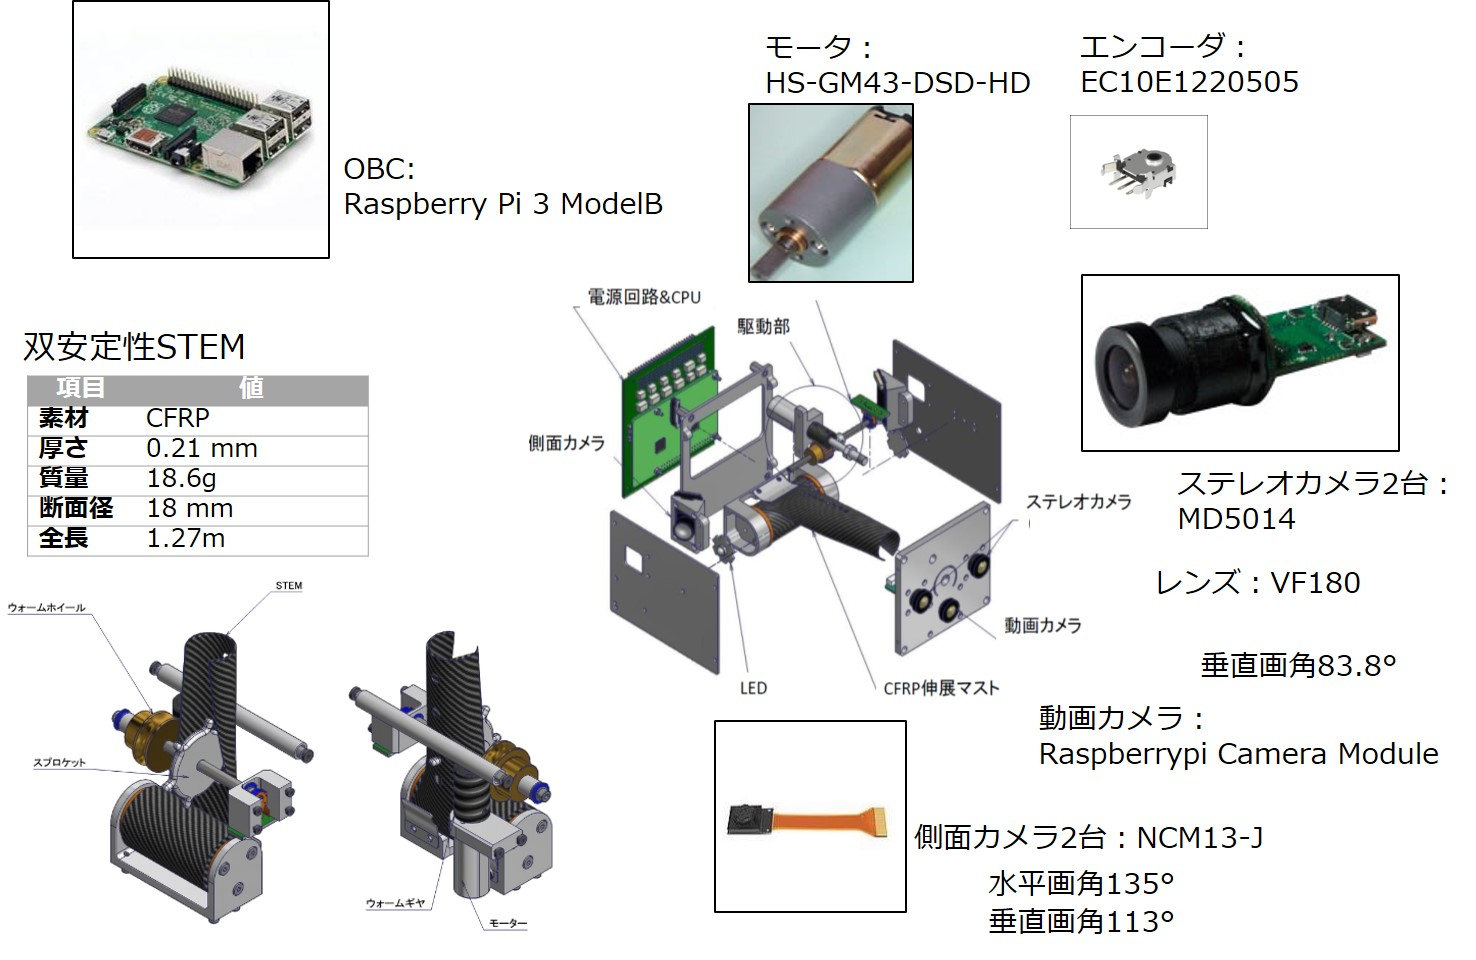
\includegraphics[width=.8\textwidth]{03/fig/3-9-2-1-1.jpg}
	\caption{伸展カメラ部の構成}
	\label{fig3-9-2-1-1}
\end{figure}
\begin{figure}[H]
	\centering
	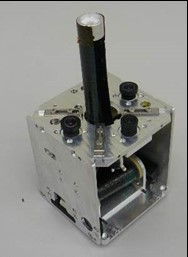
\includegraphics[width=.4\textwidth]{03/fig/3-9-2-1-2.jpg}
	\caption{伸展カメラ部EM}
	\label{fig3-9-2-1-2}
\end{figure}
\begin{figure}[H]
	\centering
	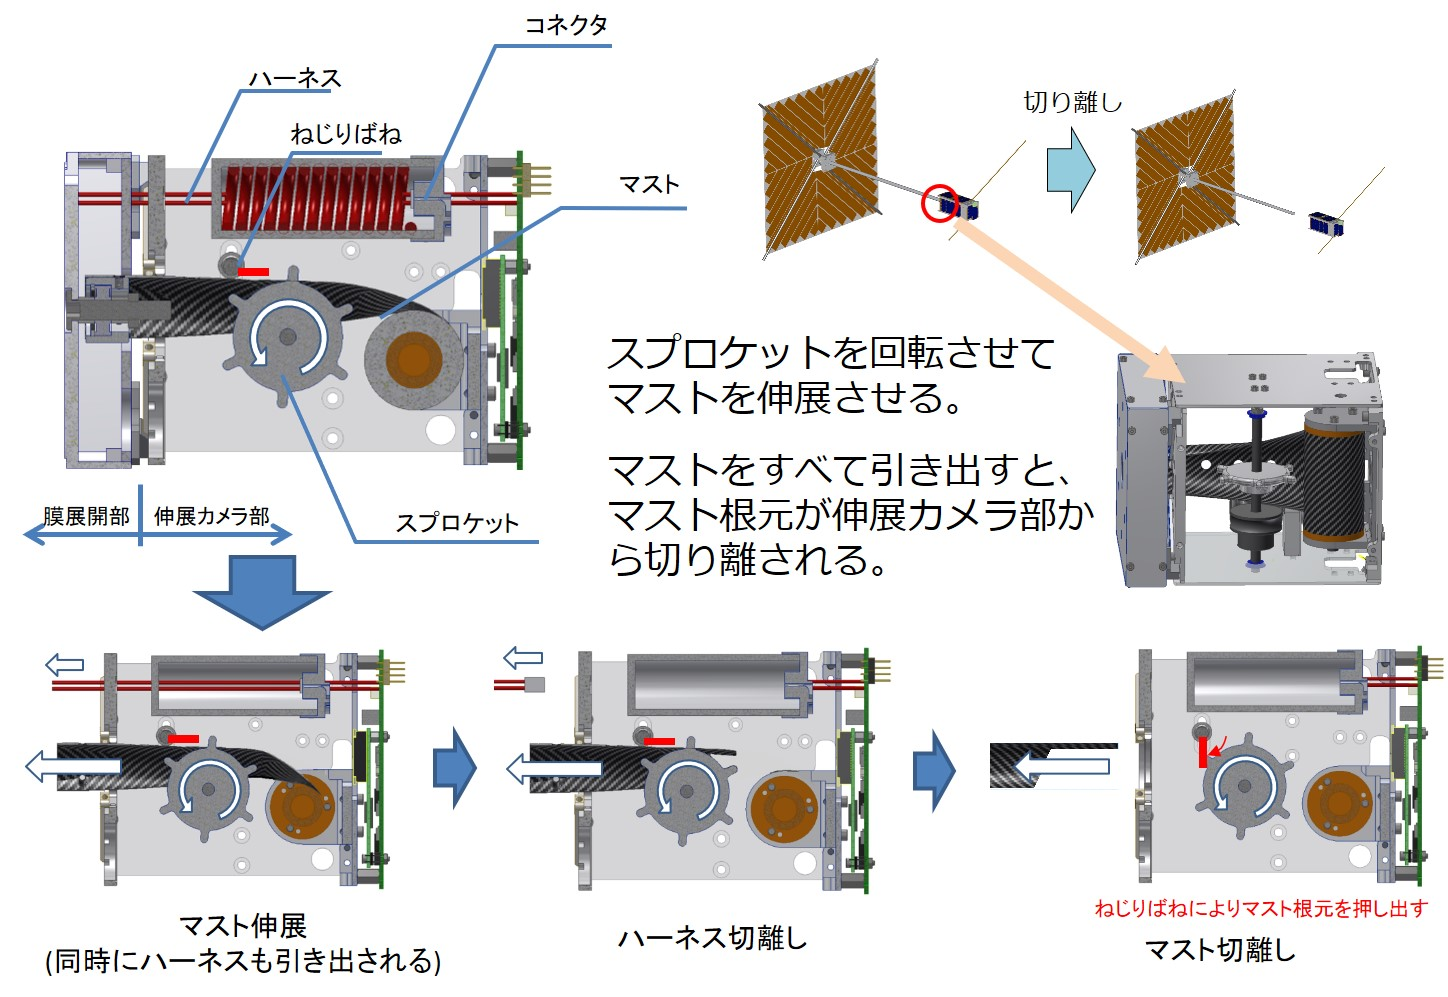
\includegraphics[width=.8\textwidth]{03/fig/3-9-2-1-3.jpg}
	\caption{伸展マストとハーネスの伸展と切り離し}
	\label{fig3-9-2-1-3}
\end{figure}

